\ifnum\solutions=1 {
  \clearpage
} \fi
\item\subquestionpoints{7}
\textbf{[Coding Problem] Semi-supervised EM Implementation.}
Now we will consider both the labelled and unlabelled examples (a total of $m + \tilde{m}$), with 5 labelled examples per cluster. We have provided starter code for splitting the dataset into a matrices \texttt{x} of labelled examples and \texttt{x\_tilde} of unlabelled examples. Add to your code in \texttt{src/p03\_gmm.py} to implement the modified EM algorithm, and run it on the dataset until convergence.

Create a plot for each trial, as done in the previous sub-question.

\textbf{Note:} You only need to submit the three plots in your write-up. Your code will not be autograded.

\ifnum\solutions=1 {
  \begin{answer}
    Please see Figure \ref{fig:sscluster}

\begin{figure}[htbp]
    \centering 
    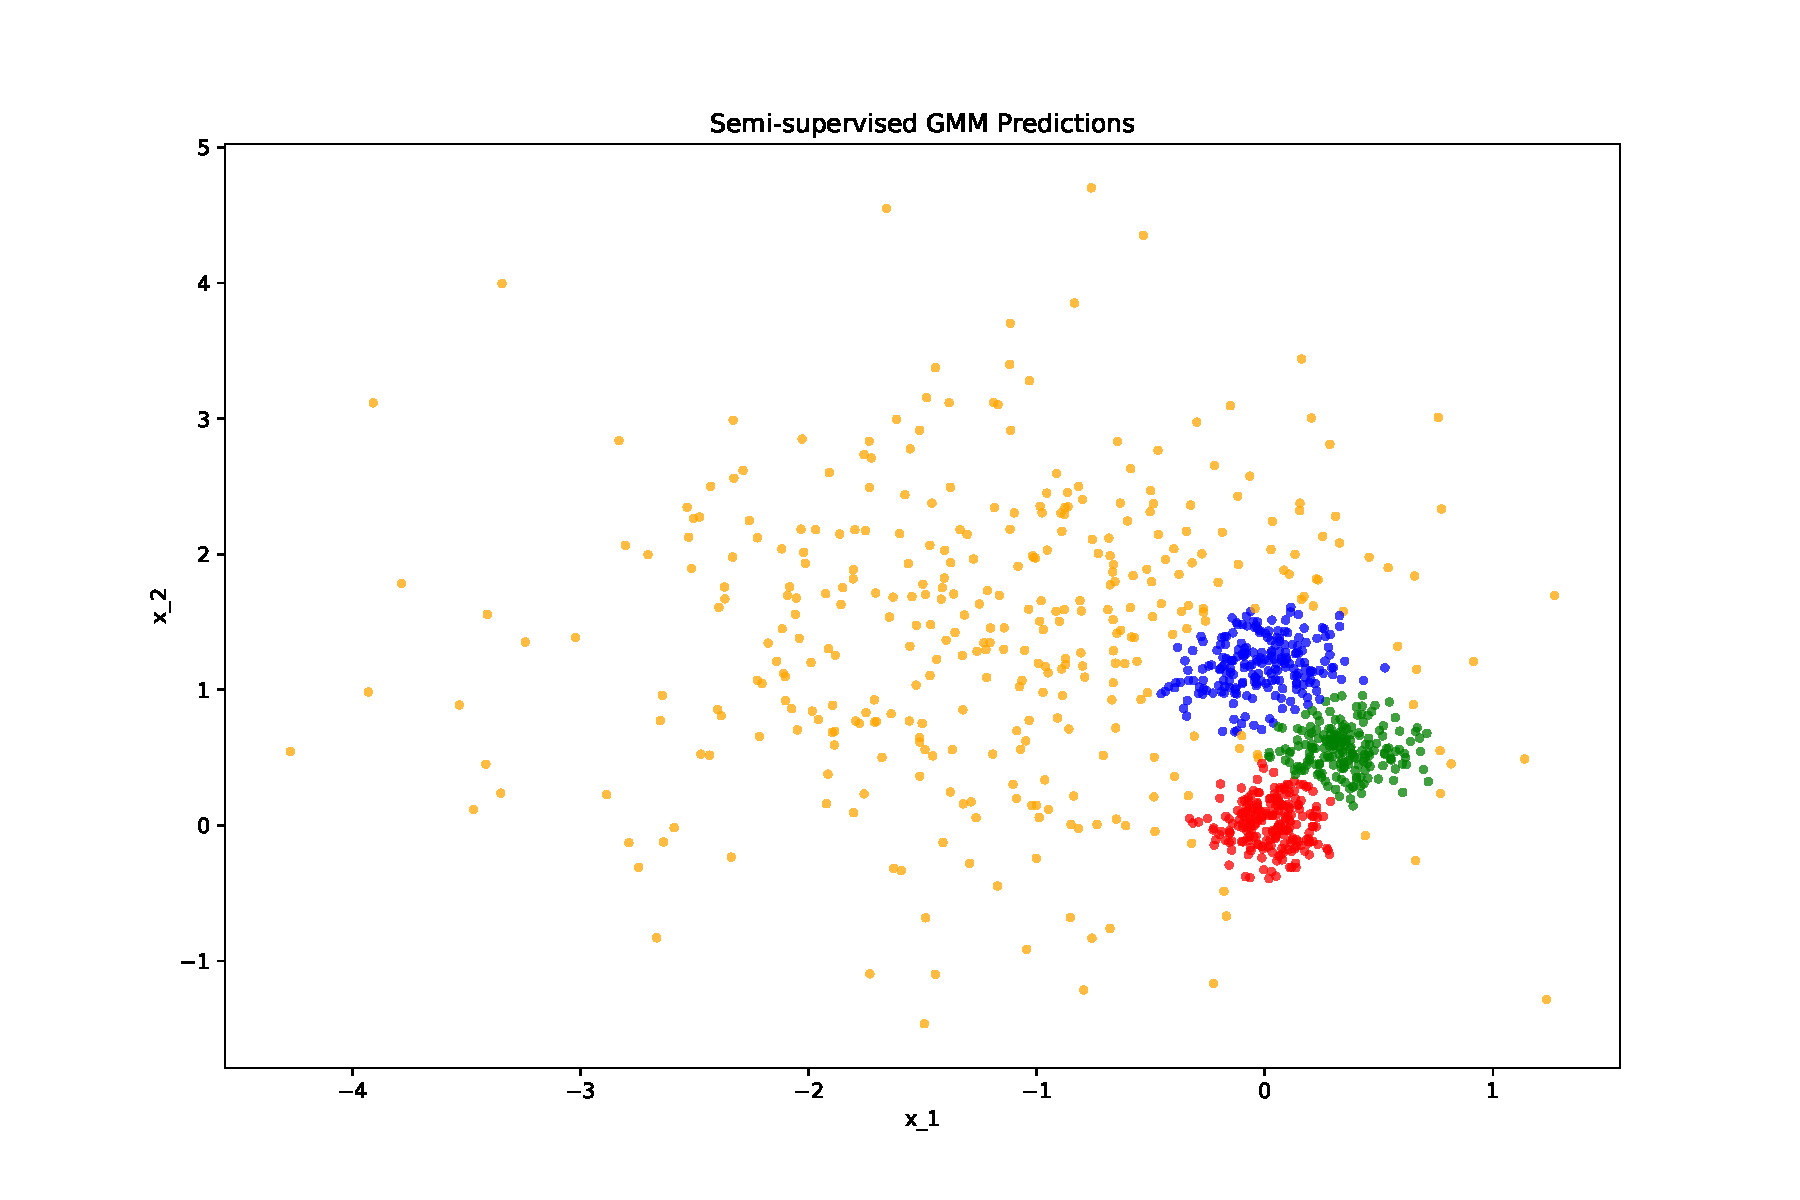
\includegraphics[width=0.7\linewidth]{pics/p03_pred_ss_0.pdf}
    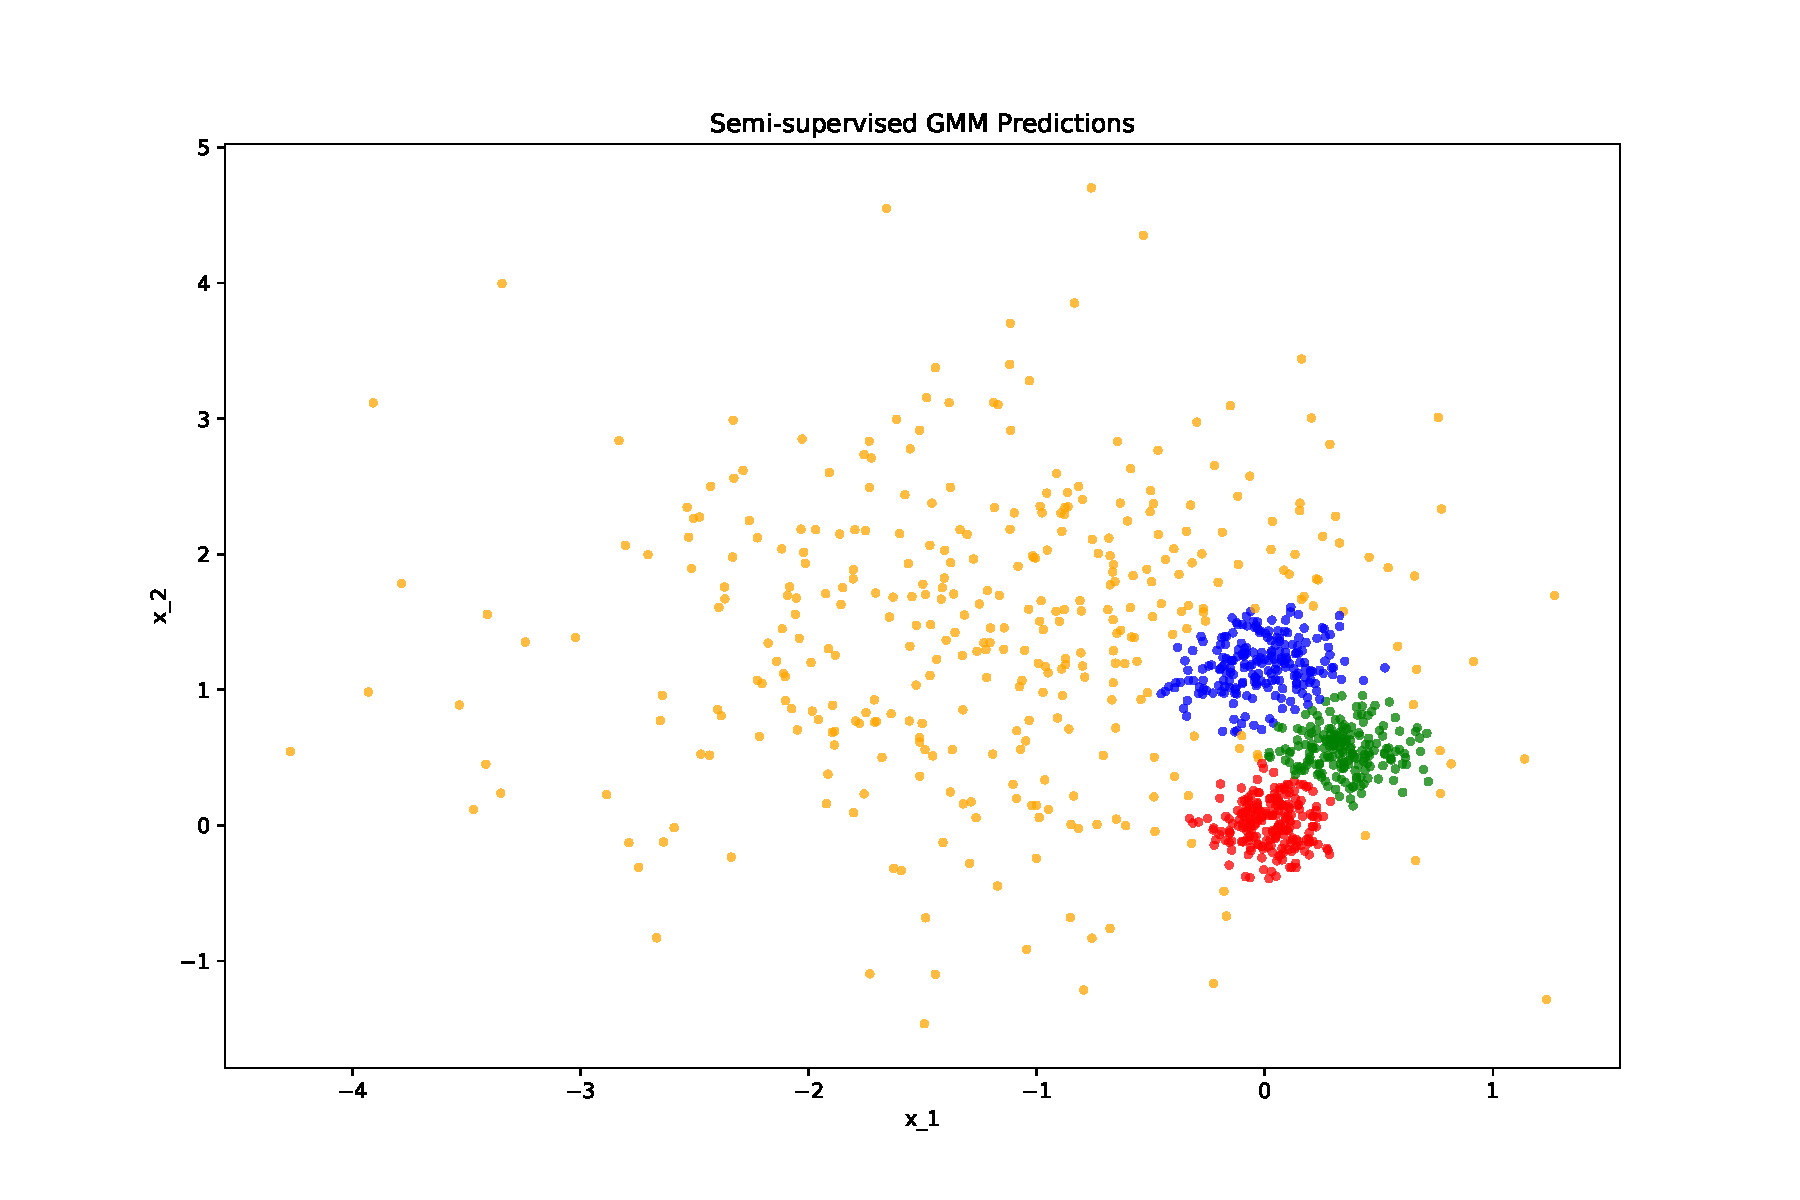
\includegraphics[width=0.7\linewidth]{pics/p03_pred_ss_1.pdf}
    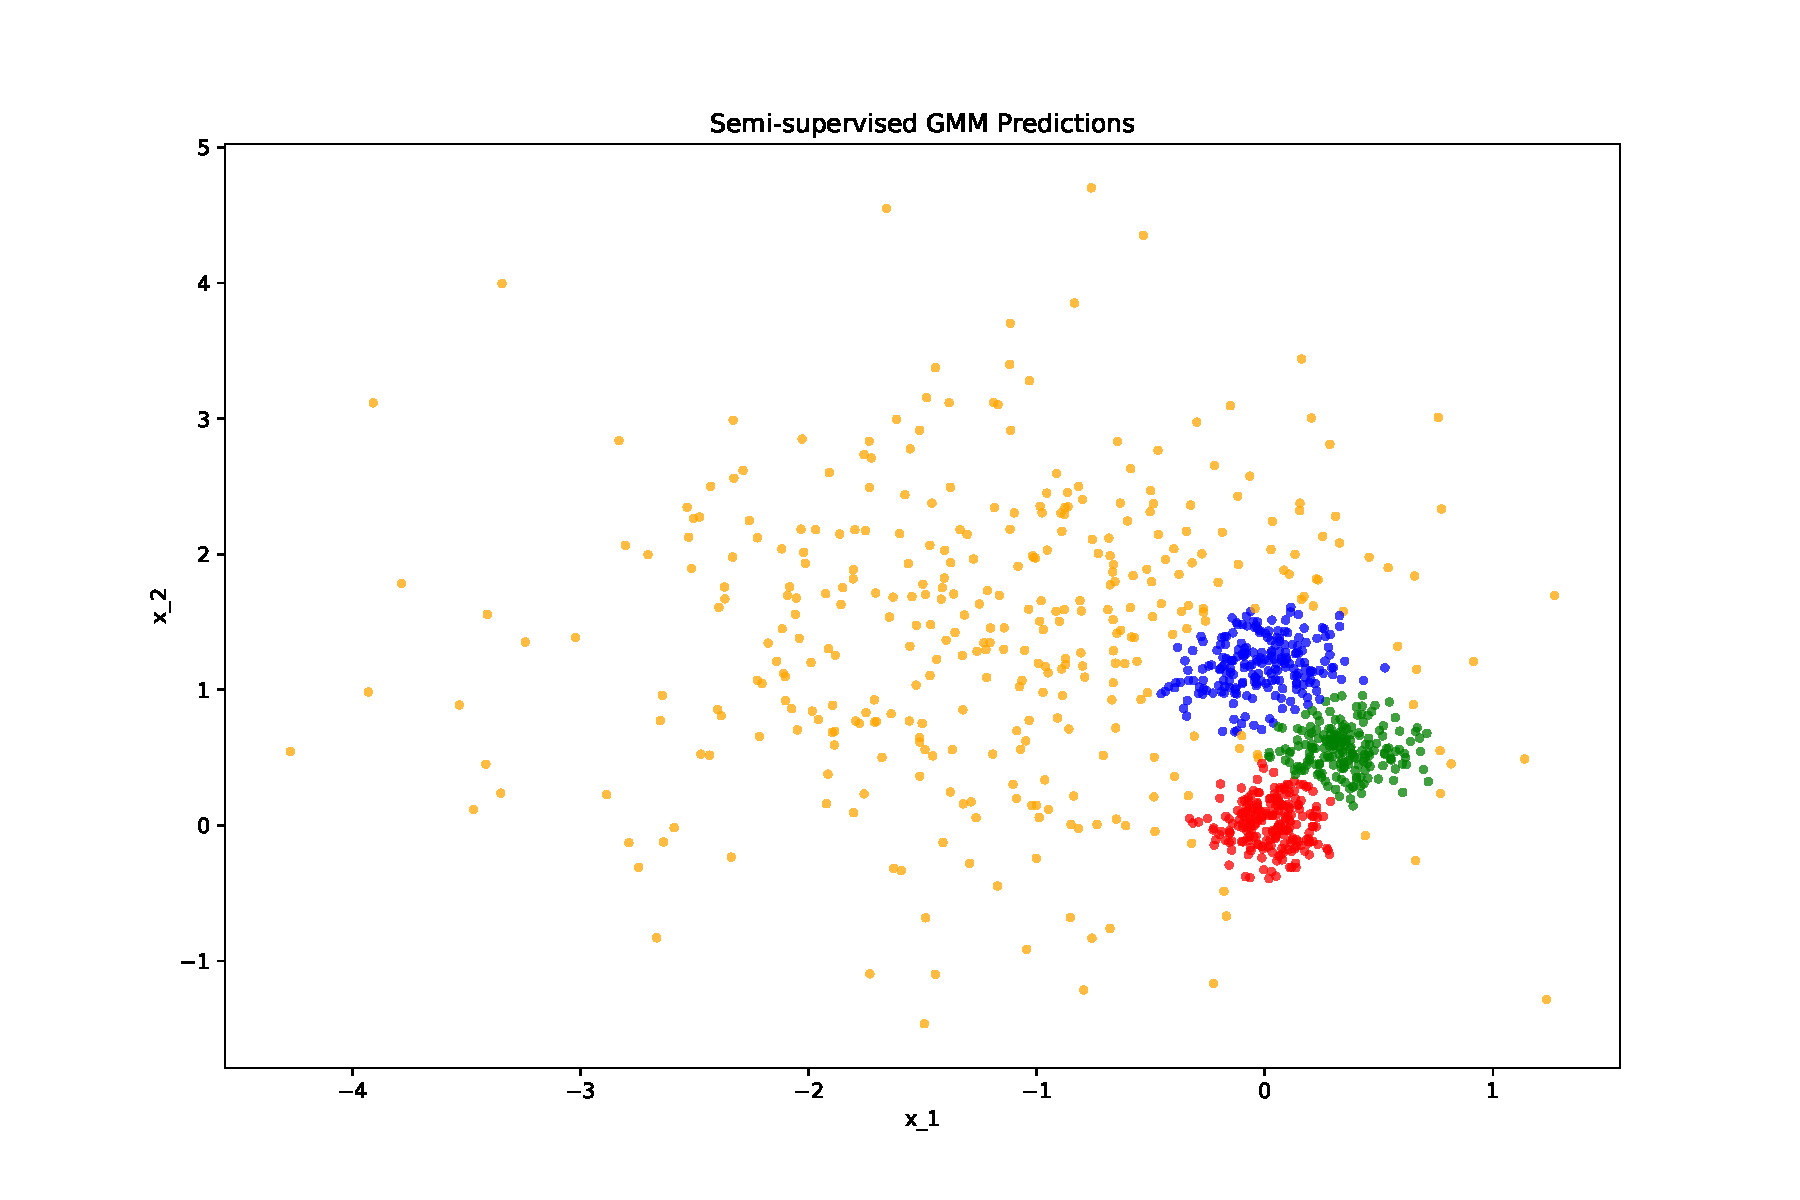
\includegraphics[width=0.7\linewidth]{pics/p03_pred_ss_2.pdf}
    \caption{Semi-Supervised Clusters}
    \label{fig:sscluster}
\end{figure}
 \end{answer}

} \fi
